% Two independent fair signs A, B and Z=AB. Each pair is uniform; the triple is not.
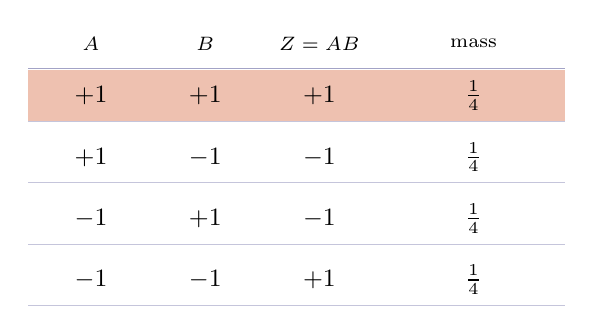
\begin{tikzpicture}[x=1.45cm,y=0.78cm]
  \draw[MidnightBlue!40] (-0.55,0.45) -- (4.15,0.45);
  \node[font=\scriptsize] at (0,0.85) {$A$};
  \node[font=\scriptsize] at (1,0.85) {$B$};
  \node[font=\scriptsize] at (2,0.85) {$Z=AB$};
  \node[font=\scriptsize] at (3.35,0.85) {mass};
  \fill[BrickRed!22] (-0.55,-0.42) rectangle (4.15,0.42);
  \foreach \r/\a/\b/\z in {0/+1/+1/+1, 1/+1/-1/-1, 2/-1/+1/-1, 3/-1/-1/+1} {
    \node[font=\small] at (0,-\r) {$\a$};
    \node[font=\small] at (1,-\r) {$\b$};
    \node[font=\small] at (2,-\r) {$\z$};
    \node[font=\small] at (3.35,-\r) {$\frac14$};
    \draw[MidnightBlue!25] (-0.55,-\r-0.42) -- (4.15,-\r-0.42);
  }
\end{tikzpicture}
